\chapter{Einleitung}\label{ch:intro}

\section{Relevanz des Themas}
Suchalgorithmen und relevante Suchergebnisse sind derzeit so relevant wie noch nie.
Dabei wollen die Benutzer einer Suchmaschine in Sekundenbruchteilen Ergebnisse, die am besten zu ihrem Suchbegriff passen, ohne sich dabei viel Gedanken über die Formulierung eines solchen Begriffes zu machen.
Ein Beispiel für einen solchen Algorithmus ist Google, welches seit den frühen 2000ern einen kometenhaften Aufstieg in der Welt der Suchmaschinen hinter sich hat, was anhand der erreichten Werbeeinnahmen sichtbar wird.\footnote{Siehe \ref{fig:werbeumsatz}}

Google ist im Vergleich zu anderen Suchmaschinen so stark verbreitet\footnote{Siehe \ref{fig:marketshare}}, dass mittlerweile sogar der Duden das Verb „googeln“ als eigenen Begriff für die Recherche im Internet führt.\footnote{Vgl. Duden \cite{duden2022}}
Dabei stellt sich für die Entwicklung eigener Produkte die Frage, wie aus einem Suchbegriff, der meist nur aus wenigen Wörtern bis zu einem ganzen Satz besteht, relevante Suchergebnisse gefunden werden können. Dies würde zur Akzeptanz der Nutzer im Hinblick auf die entwickelte Funktionalität führen, da gewünschte Ergebnisse schneller und ohne großen Aufwand gefunden werden können.

\section{Ausgangssituation}
Derzeit besteht bei \gls{crossload}\footnote{Siehe Crossload.org \cite{pfleiderer2022}}, einer Plattform zur Durchsuchung einer umfangreichen Predigtdatenbank, welche mit einer Such \gls{api} auf Basis von Spring Boot und \gls{solr} ausgestattet ist. Diese teilt auf der Suchergebnisseite die Ergebnisse nach Kategorien auf und somit können nur schwer übergreifende Suchanfragen getätigt werden. Zwar werden alle Treffer auf der gleichen Seite angezeigt, doch durch die Aufteilung nach Kategorien werden Ergebnisse gewisser Kategorien über anderen gezeigt, auch wenn niedrig positionierte Kategorien relevantere Ergebnisse enthalten.\footnote{Siehe \ref{fig:crossloadSuche}}

Durch eine Verbesserung der Relevanz, sowie einfacheres Suchen und weiterführende Vorschläge kann die Nutzerakzeptanz der Webseite weiter gefördert werden, da schneller bzw. überhaupt gesuchte Inhalte gefunden werden.
Gefundene Inhalte werden direkt auf der Crossload angehört, weswegen dadurch die mittlere Nutzungsdauer der Seite gesteigert wird.

\section{Zielsetzung \& Vorgehen}
Das Ziel der vorliegenden Studienarbeit ist es, für die oben genannte Problemstellung einen Prototyp zur Erweiterung und Verbesserung des bisher genutzten Suchalgorithmus bei Crossload zu entwickeln.

Einleitend wird ein Einblick in die Grundlagen der Relevanz sowie mögliche Methoden und Funktionen zur Bewertung gegeben, sowie auf eine finale Auswertung der gesammelten Methoden eingegangen.
Die hier erarbeiteten Grundlagen und Methoden werden im weiteren Verlauf mit in die Entwicklung einfließen.
Anschließend folgt eine kurze Einleitung zu SOLR, der genutzten Search Engine von Crossload.
Dieser theoretische Teil der Arbeit basiert größtenteils auf einer Literaturrecherche.
Google Scholar, relevante Dokumentationen oder die einfache Google Suche stellen dazu die Grundlage dar.
Die gefundenen Ergebnisse werden auf Qualität und Themenbezug geprüft.

Anhand der gegebenen Aufgabenstellung werden Anforderungen nach dem SMART Prinzip\footnote{Vgl. Witte 2019a, S. 67 \cite{witte2016}} erarbeitet, die als Grundlage der darauffolgenden Konzeption und Entwicklung dienen sollen.
Ebenso werden bereits etablierte Tools genutzt, um die Anforderungen weiter zu verfeinern.

Für die Entwicklung wird dabei das Wasserfallmodell genutzt.
Obwohl es in seinen Nachteilen gegenüber z. B. agilen Methoden überwiegt, bietet es doch wenig Aufwand um die eigentliche Entwicklung herum und stellt eine klare Struktur bereit.
Diese hilft, schnell ein Produkt, oder in diesem Fall einen Prototyp, fertigzustellen.
Das Modell ist auch vorteilhaft, weil die Anforderungen in ihrer Gesamtheit schon bekannt sind, beziehungsweise vor der Entwicklung sein werden und keine weiteren Faktoren hinzukommen. Die dafür verwendeten Phasen, Anforderungserhebung, Entwicklung und anschließendem Test der Anforderungen, werden in nachfolgender Abbildung verdeutlicht.
\begin{figure}[h]
  \begin{centering}
    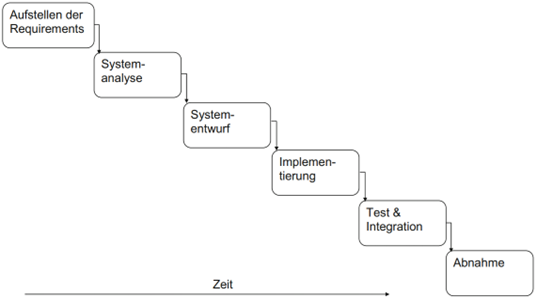
\includegraphics[width=.6\textwidth]{figures/intro/waterfall.png}
    \caption{Grundform eines Wasserfallmodells ohne Machbarkeitsanalyse. Nach Goll \cite{goll2011}.}
    \label{fig:waterfall}
  \end{centering}
\end{figure}

Im Rahmen der Konzeption wird auf die bisherige Funktionalität eingegangen, um mögliche Probleme und Verbesserungspotenzial aufzudecken. Anschließend wird eine neue Berechnung des Relevanzscores mithilfe der erarbeiteten Methoden zur Berechnung der Relevanz geplant. Die Konzeption wird abgeschlossen mit der Planung der Entwicklung, mit welcher die gesammelten Anforderungen umgesetzt werden sollen.

Die Implementierung umfasst, die nach Kontext und Wahrscheinlichkeiten gewichtete und gefilterte Suche über eine Datenbank mit Datentypen verschiedener Kategorien bei der zusätzlich Vorschläge zur weiteren Navigation auf der Suchergebnisseite gegeben werden sollen.

Schlussendlich werden die Ergebnisse der Entwicklung zusammengefasst, die Anforderungen und die Implementation bewertet, sowie durch einen Ausblick, wie der Prototyp in einen produktiven Betrieb übergehen könnte, und ein Fazit abgerundet.

Im Lauf der Arbeit werden die folgenden Fragen beantwortet:
\begin{itemize}
  \item Was ist Relevanz?
  \item Wie wird Relevanz in Suchmaschinen berechnet bzw. bewertet?
  \item Welche Anforderungen ergeben sich an ein solches Plugin?
  \item Mit welchen Methoden kann die aktuelle Implementierung verbessert werden?
  \item Welche Vorteile, Nachteile oder Hürden bringt die Implementation mit sich?
\end{itemize}
